\documentclass{exam}
\usepackage[utf8]{inputenc}
\usepackage{graphicx}
\usepackage{tikz}
\usepackage[margin=2cm]{geometry}
%\geometry{
%  left=3cm,
%  top=3cm,
%}
%	\addtolength{\oddsidemargin}{-.875in}
%	\addtolength{\evensidemargin}{-.875in}
%	\addtolength{\textwidth}{1.75in}
%
	%\addtolength{\topmargin}{1cm}
	%\addtolength{\rightmargin}{1cm}
%	\addtolength{\textheight}{1.75in}
\begin{document}

%\begin{center}
%\fbox{\fbox{\parbox{5.5in}{\centering
%Answer the questions in the spaces provided. If you run out of room
%for an answer, continue on the back of the page.}}}
%\end{center}
%\vspace{5mm}
%\vspace{xcm}
    %\vspace{3cm}
    %\hspace{3cm}
%\vspace{5mm}
%\makebox[\textwidth]{Instructor’s name:\enspace\hrulefill}
\makebox[\dimexpr\textwidth][r]{
\includegraphics[height=1.5cm]{./images/marca-udesc.png}} 
\makebox[\textwidth]{Nome: \enspace\hrulefill, Turma: 1º F}

\begin{questions}
    \question Seja $f(x) = 2^{x+1}$. 
    \begin{parts}
        \part[2] Encontre a função inversa.
        \part[2] Esboce o gráfico de ambas usando o plano representado logo abaixo. \\
            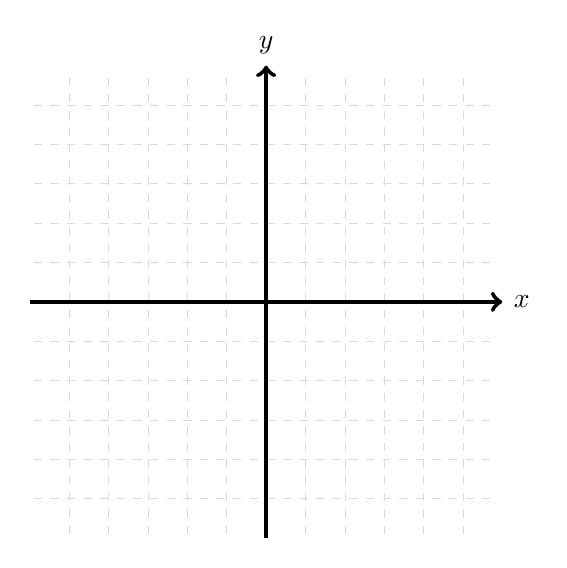
\begin{tikzpicture}[scale=0.5]
            \draw[help lines, color=gray!30, dashed] (-5.9,-5.9) grid (5.9,5.9);
            \draw[->,ultra thick] (-6,0)--(6,0) node[right]{$x$};
            \draw[->,ultra thick] (0,-6)--(0,6) node[above]{$y$};
        \end{tikzpicture}
    \end{parts}

    \question Considere um título LCI (Letra de Crédito Imobiliário) de renda fixa de $10\%$ a.a.
    \begin{parts}
      \part[1]  Calcule quanto uma aplicação de $R\$ 1000$ rende em cada ano, durante $5$ anos.
      \part[1]  Esboce o gráfico do montante desta aplicação usando o plano representado logo abaixo. \\
      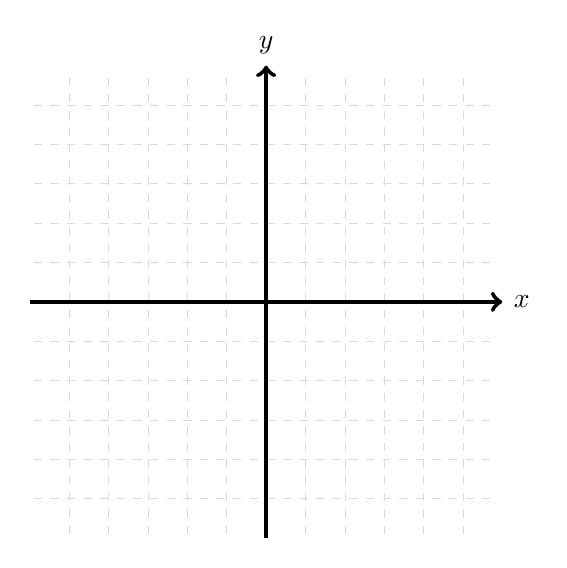
\begin{tikzpicture}[scale=0.5]
          \draw[help lines, color=gray!30, dashed] (-5.9,-5.9) grid (5.9,5.9);
          \draw[->,ultra thick] (-6,0)--(6,0) node[right]{$x$};
          \draw[->,ultra thick] (0,-6)--(0,6) node[above]{$y$};
      \end{tikzpicture}
      \part[1.5]  Quando o montante é $R\$ 2000$?
    \end{parts}

    \question Um determinado programa de computador inicia seu processo com $1Mb$ de memória RAM.
    Sabe-se que sempre que ele precisa de mais memória ele requisita (ao Sistema Operacional) 
    a quantidade de memória que tem no momento da requisição. Por exemplo, se ele tem $3Mb$
    de memória e necessita de mais, ele requisita mais $3Mb$, ficando com $6Mb$ (donde $3Mb$ estão ocupados e $3Mb$ livres).
    José, identifica que o programa está usando $50Mb$.
    \begin{parts}
        \part[1.5] Quantas vezes o programa solicitou memória ao Sistema Operacional?
        \part[1] Quanto de memória ele tem ainda disponível sem precisar solicitar mais?
    \end{parts}
\end{questions}
\end{document}
